% block: machine-learning-heading page:68 type:section
\subsection{{机器学习}}\label{sec:machine-learning}
{机器学习领域也会产生线性方程组. 本节通过最小二乘回归和最小二乘分类两个例子, 说明线性方程组的重要性.}
% block: least-squares-regression-heading page:68 type:subsection
\subsubsection{{最小二乘回归}}\label{subsec:least-squares-regression}
{本小节考虑最简单的监督学习之一: 最小二乘学习. 给定训练数据集 \linebreak[4]$(\boldsymbol{x}_i,y_i)$ ($i=1,\ldots,n$) 和函数 $f_{\boldsymbol{\theta}}(\boldsymbol{x})$. 最小二乘学习要学习一个参数 $\boldsymbol{\theta}\in\mathbb{R}^m$, 使下列误差函数达到极小值:}
\begin{equation}\label{eq:least-squares-loss}
J(\boldsymbol{\theta})=\sum_{i=1}^n(y_i-f_{\boldsymbol{\theta}}(\boldsymbol{x}_i))^2.
\end{equation}
{若 $f_{\boldsymbol{\theta}}(\boldsymbol{x})$ 由函数 $f_1(\boldsymbol{x}),\ldots,f_m(\boldsymbol{x})$ 的线性组合给出, 形式为}
\begin{equation}\label{eq:regression-basis-model}
f_{\boldsymbol{\theta}}(\boldsymbol{x})=\theta_1f_1(\boldsymbol{x})+\theta_2f_2(\boldsymbol{x})+\theta_mf_m(\boldsymbol{x}),
\end{equation}
{则误差函数 \eqref{eq:least-squares-loss} 可改写为}\footnote{{本节将 2-范数明确写成 $\|\cdot\|_2$. 机器学习中也使用 1-范数 $\|\cdot\|_1$, 尤其用于得到形如 $\|\boldsymbol{y}-M\boldsymbol{\theta}\|_2^2+\lambda\|\boldsymbol{\theta}\|_1$ 的最小二乘问题的稀疏解.}}
\begin{equation}\label{eq:least-squares-matrix-loss}
J(\boldsymbol{\theta})=\|\boldsymbol{y}-M\boldsymbol{\theta}\|_2^2,
\end{equation}
{其中 $\boldsymbol{y}=[y_1,y_2,\ldots,y_n]^{\top}$, $\boldsymbol{\theta}=[\theta_1,\theta_2,\ldots,\theta_m]^{\top}$, 且}
% block: regression-design-matrix page:69 type:ordinary-paragraph
\[M=\begin{bmatrix}
f_1(\boldsymbol{x}_1)&f_2(\boldsymbol{x}_1)&\cdots&f_m(\boldsymbol{x}_1)\\
f_1(\boldsymbol{x}_2)&f_2(\boldsymbol{x}_2)&\cdots&f_m(\boldsymbol{x}_2)\\
\vdots&\vdots&\ddots&\vdots\\
f_1(\boldsymbol{x}_n)&f_2(\boldsymbol{x}_n)&\cdots&f_m(\boldsymbol{x}_n)
\end{bmatrix}.\]
{为简单起见, 假设 $M$ 的列向量线性无关. 为使误差函数 \eqref{eq:least-squares-matrix-loss} 达到极小值, 下列分解很有用:}
\begin{equation}\label{eq:least-squares-square-completion}
\begin{aligned}
J(\boldsymbol{\theta})&=\|\boldsymbol{y}-M\boldsymbol{\theta}\|_2^2=(\boldsymbol{y}-M\boldsymbol{\theta})^{\top}(\boldsymbol{y}-M\boldsymbol{\theta})\\
&=\boldsymbol{v}_{\boldsymbol{\theta}}^{\top}(M^{\top}M)^{-1}\boldsymbol{v}_{\boldsymbol{\theta}}-(M^{\top}\boldsymbol{y})^{\top}(M^{\top}M)^{-1}(M^{\top}\boldsymbol{y})+\boldsymbol{y}^{\top}\boldsymbol{y}.
\end{aligned}
\end{equation}
{这里 $\boldsymbol{v}_{\boldsymbol{\theta}}=M^{\top}\boldsymbol{y}-M^{\top}M\boldsymbol{\theta}$. 由于 $M$ 的列线性无关, $M^{\top}M$ 为对称正定矩阵, 即所有特征值均为正, 或等价地, 对所有非零向量 $\boldsymbol{x}$, 有 $\boldsymbol{x}^{\top}M^{\top}M\boldsymbol{x}>0$. 由此, 若 $\boldsymbol{v}_{\boldsymbol{\theta}}=\boldsymbol{0}$, 即 $M^{\top}\boldsymbol{y}-M^{\top}M\boldsymbol{\theta}=\boldsymbol{0}$, 则 $J(\boldsymbol{\theta})$ 达到极小值. 因此需要求解下列线性方程组:}
\begin{equation}\label{eq:regression-normal-equations}
M^{\top}M\boldsymbol{\theta}=M^{\top}\boldsymbol{y}.
\end{equation}
% block: regression-example page:69 type:ordinary-paragraph
{作为数值例子, 考虑 $y=(1/2)\sin(x)+\epsilon$, 其中 $\epsilon$ 为噪声. 我们取 \linebreak[4]$(x_1,x_2,\ldots,x_{63})=(0,0.1,0.2,\ldots,6.2)$ 和 \linebreak[4]$(y_1,y_2,\ldots,y_{63})=(y(0),y(0.1),y(0.2),\ldots,y(6.2))$ 生成一个数据集 (训练数据集). 数据的可视化结果见 Fig.\ \ref{fig:regression-data}.}
{接着考虑 \eqref{eq:regression-basis-model}. 对基函数 $f_1(x),f_2(x),\ldots,f_m(x)$, 使用}
\[f_k(x)=\begin{cases}\sin\frac12kx&(k:\text{even}),\\\cos\frac12kx&(k:\text{odd}).\end{cases}\]
{模型函数 \eqref{eq:regression-basis-model} 的未知向量 $\boldsymbol{\theta}$ 通过求解线性方程组 \eqref{eq:regression-normal-equations} 得到, $m=5$ 和 $m=10$ 时 $f_{\boldsymbol{\theta}}(x)$ 的图像见 Fig.\ \ref{fig:regression-fit}.}
% block: regression-data-figure page:69 type:figure
\begin{figure}[htbp]\centering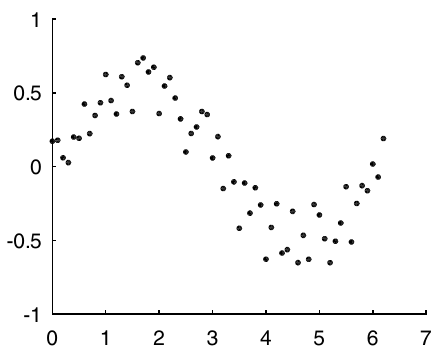
\includegraphics[width=.48\linewidth]{figures/regression-data.png}
\caption{{给定数据集的图像}}\label{fig:regression-data}\end{figure}
% block: regression-fit-figure page:70 type:figure
\begin{figure}[htbp]\centering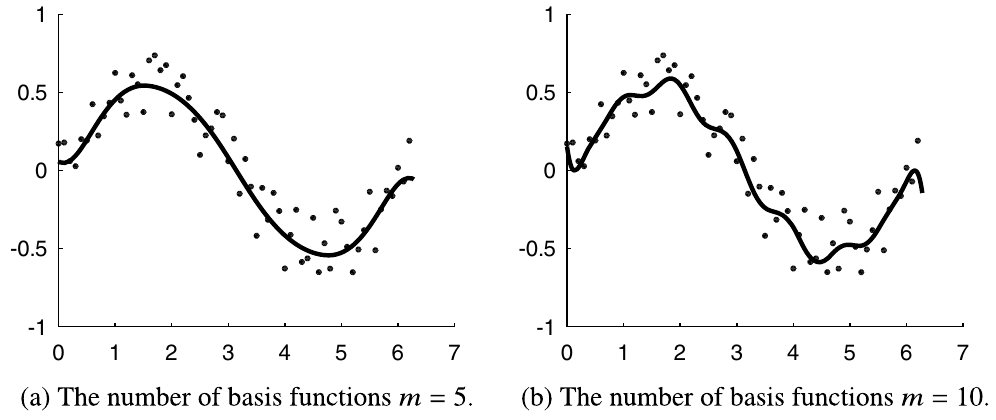
\includegraphics[width=.92\linewidth]{figures/regression-fit.png}
\caption{{\eqref{eq:regression-basis-model} 中 $m=5$ 和 $m=10$ 时 $f_{\boldsymbol{\theta}}(x)$ 的图像. (a) 基函数个数 $m=5$. (b) 基函数个数 $m=10$.}}\label{fig:regression-fit}\end{figure}
% block: regression-overfitting page:70 type:ordinary-paragraph
{由 Fig.\ \ref{fig:regression-fit}a 可见, $m=5$ 时函数 $f_{\boldsymbol{\theta}}(x)$ 对噪声具有鲁棒性. 另一方面, $m=10$ 时的函数似乎试图拟合含给定噪声的数据. 这一现象称为过拟合.}
{下面介绍一种克服过拟合的方法, 它同样需要求解 (参数化的) 线性方程组. 现在考虑下列形式的约束极小化问题}
\begin{equation}\label{eq:constrained-regression}
\min_{\boldsymbol{\theta}}\|\boldsymbol{y}-M\boldsymbol{\theta}\|_2^2\quad\text{subject to }\|\boldsymbol{\theta}\|_2^2\le R.
\end{equation}
{若 $R$ 为无穷大, 则该极小化问题等价于 \eqref{eq:least-squares-matrix-loss}. 为求解 \eqref{eq:constrained-regression}, 对偶问题很有用. 令 $f(\boldsymbol{\theta})=\|\boldsymbol{y}-M\boldsymbol{\theta}\|_2^2$, $g(\boldsymbol{\theta})=\|\boldsymbol{\theta}\|_2^2-R$, 则 \eqref{eq:constrained-regression} 可改写为}
\begin{equation}\label{eq:abstract-constrained-regression}
\min_{\boldsymbol{\theta}}f(\boldsymbol{\theta})\quad\text{subject to }g(\boldsymbol{\theta})\le0.
\end{equation}
{这里对 $\lambda\ge0$ 引入 Lagrange 函数:}
\[L(\boldsymbol{\theta},\lambda):=f(\boldsymbol{\theta})+\lambda g(\boldsymbol{\theta}).\]
{由于 $\lambda\ge0$ 且 $g(\boldsymbol{\theta})\le0$, 有}
\[\max_{\lambda\ge0}L(\boldsymbol{\theta},\lambda)=\begin{cases}f(\boldsymbol{\theta})&\text{(if }g(\boldsymbol{\theta})\le0),\\+\infty&\text{(otherwise)}.\end{cases}\]
{因此 \eqref{eq:abstract-constrained-regression} 等价于}
\[\min_{\boldsymbol{\theta}}\max_{\lambda\ge0}L(\boldsymbol{\theta},\lambda).\]
% block: regression-duality page:71 type:ordinary-paragraph
{现在考虑下列对偶问题:}
\begin{equation}\label{eq:regression-dual-problem}
\max_{\lambda\ge0}\min_{\boldsymbol{\theta}}L(\boldsymbol{\theta},\lambda).
\end{equation}
{若 $f$ 和 $g$ 是凸的, 并满足一定条件, 则有}
\[\max_{\lambda\ge0}\min_{\boldsymbol{\theta}}L(\boldsymbol{\theta},\lambda)=\min_{\boldsymbol{\theta}}\max_{\lambda\ge0}L(\boldsymbol{\theta},\lambda),\]
{这称为强对偶性, 与 Lagrangian 对偶理论有关; 详情见 \BookCite{26}. 优化问题 \eqref{eq:regression-dual-problem} 为}
\begin{equation}\label{eq:regularized-regression-dual}
\max_{\lambda\ge0}\min_{\boldsymbol{\theta}}L(\boldsymbol{\theta},\lambda)\Leftrightarrow
\max_{\lambda\ge0}\min_{\boldsymbol{\theta}}\|\boldsymbol{y}-M\boldsymbol{\theta}\|_2^2+\lambda(\|\boldsymbol{\theta}\|_2^2-R).
\end{equation}
% block: regularized-square-completion page:71 type:ordinary-paragraph
{与 \eqref{eq:least-squares-square-completion} 类似, 误差函数可分解为}
\[\begin{aligned}
&\|\boldsymbol{y}-M\boldsymbol{\theta}\|_2^2+\lambda(\|\boldsymbol{\theta}\|_2^2-R)\\
&=\boldsymbol{w}_{\boldsymbol{\theta}}^{\top}(M^{\top}M+\lambda I)^{-1}\boldsymbol{w}_{\boldsymbol{\theta}}-(M^{\top}\boldsymbol{y})^{\top}(M^{\top}M+\lambda I)^{-1}M^{\top}\boldsymbol{y}+\boldsymbol{y}^{\top}\boldsymbol{y}-\lambda R,
\end{aligned}\]
{其中 $\boldsymbol{w}_{\boldsymbol{\theta}}=M^{\top}\boldsymbol{y}-(M^{\top}M+\lambda I)\boldsymbol{\theta}$. 由于 $\lambda\ge0$, 矩阵 $M^{\top}M+\lambda I$ 为对称正定矩阵. 因此可通过求解下列线性方程组得到 $\boldsymbol{\theta}$:}
\begin{equation}\label{eq:regularized-normal-equations}
(M^{\top}M+\lambda I)\boldsymbol{\theta}=M^{\top}\boldsymbol{y}.
\end{equation}
{设 $\boldsymbol{\theta}(\lambda)$ 为线性方程组 \eqref{eq:regularized-normal-equations} 的解. 则 \eqref{eq:regression-dual-problem} 等价于}
\[\max_{\lambda\ge0}L(\boldsymbol{\theta}(\lambda),\lambda).\]
{为近似求解上述极大化问题, 可取 $0\le\lambda_1<\lambda_2<\cdots<\lambda_m$, 然后计算}
\[\max\{L(\boldsymbol{\theta}(\lambda_1),\lambda_1),L(\boldsymbol{\theta}(\lambda_2),\lambda_2),\ldots,L(\boldsymbol{\theta}(\lambda_m),\lambda_m)\}.\]
{此时需要 $\boldsymbol{\theta}(\lambda_1),\boldsymbol{\theta}(\lambda_2),\ldots,\boldsymbol{\theta}(\lambda_m)$, 即}
\begin{equation}\label{eq:regression-shifted-systems}
(M^{\top}M+\lambda_k I)\boldsymbol{\theta}(\lambda_k)=M^{\top}\boldsymbol{y}\quad k=1,2,\ldots,m.
\end{equation}
{方程 \eqref{eq:regression-shifted-systems} 称为移位线性方程组. 求解移位线性方程组的 Krylov 子空间方法将在 Chapter\ \ref{chap:shifted-linear-systems} 中介绍.}
% block: regularization-numerical-example pages:71,72 type:ordinary-paragraph
{下面给出一个数值例子, 数据与 Fig.\ \ref{fig:regression-data} 相同. 给定 $\lambda$, 求解线性方程组 \eqref{eq:regularized-normal-equations}, 得到模型函数 \eqref{eq:regression-basis-model} 的未知向量 $\boldsymbol{\theta}$. $m=10$, $\lambda=1.0$ 时 $f_{\boldsymbol{\theta}}(x)$ 的图像见 Fig.\ \ref{fig:regularized-regression-fit}b. 为便于对照, 在 Fig.\ \ref{fig:regularized-regression-fit}a 中再次给出 Fig.\ \ref{fig:regression-fit}b.}
{由 Fig.\ \ref{fig:regularized-regression-fit}b 可见, 结果现在对噪声具有鲁棒性, 因而似乎避免了 Fig.\ \ref{fig:regularized-regression-fit}a 中出现的过拟合.}
% block: regularized-regression-fit-figure page:72 type:figure
\begin{figure}[htbp]\centering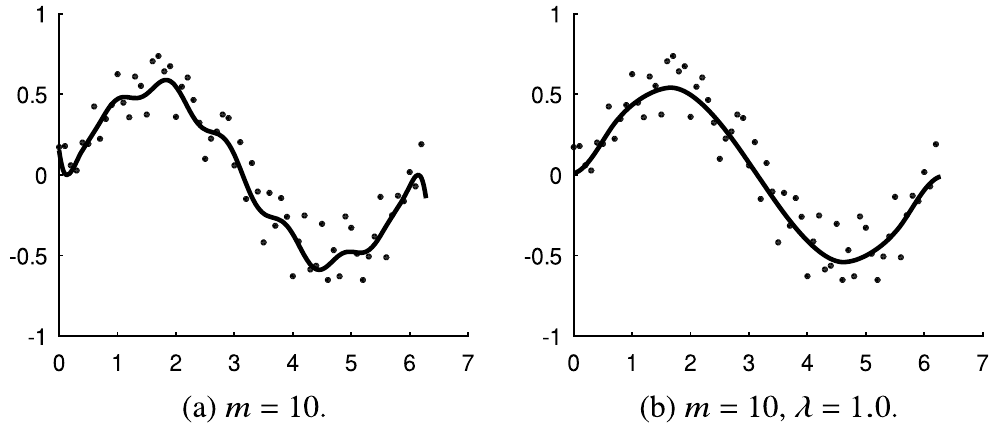
\includegraphics[width=.92\linewidth]{figures/regularized-regression-fit.png}
\caption{{\eqref{eq:regression-basis-model} 中 $m=10$ 及 $m=10$, $\lambda=1.0$ 时 $f_{\boldsymbol{\theta}}(x)$ 的图像. (a) $m=10$. (b) $m=10$, $\lambda=1.0$.}}\label{fig:regularized-regression-fit}\end{figure}
% block: probabilistic-classification-heading page:72 type:subsection
\subsubsection{{最小二乘分类}}\label{subsec:least-squares-classification}
{本小节介绍最小二乘概率分类 \BookCite{178} (概述亦见 \BookCite{148}).}
{设 $\mathcal{X}\subset\mathbb{R}^d$, $\mathcal{Y}=\{1,2,\ldots,c\}$, 其中 $c$ 为类别数. 分类问题是依据给定的数据集 (训练数据集) $(\boldsymbol{x}_i,y_i)\in\mathcal{X}\times\mathcal{Y}$ ($i=1,2,\ldots,n$), 将 $\boldsymbol{x}\in\mathcal{X}$ 分入类别 $y\in\mathcal{Y}$. 这里 $(\boldsymbol{x}_i,y_i)$ 表示数据 $\boldsymbol{x}_i\in\mathcal{X}$ 属于类别 $y_i\in\mathcal{Y}$.}
{概率模式识别是根据训练数据 $\{(\boldsymbol{x}_i,y_i)\}_{i=1}^n$ 估计类别后验概率 $p(y|\boldsymbol{x})$. 一旦得到 $p(y|\boldsymbol{x})$, 新数据 $\boldsymbol{x}$ 即可按下式分类}
\[\widehat y=\operatorname*{arg\,max}_{y\in\{1,2,\ldots,c\}}p(y|\boldsymbol{x}).\]
{设 $p(\boldsymbol{x})$ 为 $\boldsymbol{x}$ 的边缘密度, 且对所有 $\boldsymbol{x}$ 满足 $p(\boldsymbol{x})>0$. 则类别后验概率 $p(y|\boldsymbol{x})$ 可写为}
\begin{equation}\label{eq:class-posterior-probability}
p(y|\boldsymbol{x})=\frac{p(\boldsymbol{x},y)}{p(\boldsymbol{x})},
\end{equation}
{这是因为 $p(\boldsymbol{x},y)=p(y|\boldsymbol{x})p(\boldsymbol{x})$, 并且假设 $p(\boldsymbol{x})>0$. 最小二乘概率分类对类别后验概率 $p(y|\boldsymbol{x})$ 使用下列线性模型 $q(y|\boldsymbol{x};\boldsymbol{\theta}^{(y)})$:}
% block: classification-model page:73 type:ordinary-paragraph
\begin{equation}\label{eq:classification-basis-model}
q(y|\boldsymbol{x};\boldsymbol{\theta}^{(y)})=\boldsymbol{\theta}^{(y)\top}\boldsymbol{f}(\boldsymbol{x})=\theta_1^{(y)}f_1(\boldsymbol{x})+\theta_2^{(y)}f_2(\boldsymbol{x})+\cdots+\theta_b^{(y)}f_b(\boldsymbol{x}),
\end{equation}
{其中 $\boldsymbol{\theta}^{(y)}=[\theta_1^{(y)},\theta_2^{(y)},\ldots,\theta_b^{(y)}]^{\top}$, $f_i(\boldsymbol{x})$ ($i=1,\ldots,b$) 为给定基函数, 例如}
\begin{equation}\label{eq:classification-gaussian-kernel}
f_i(\boldsymbol{x})=K(\boldsymbol{x},\boldsymbol{x}_i)=\exp\left(-\frac{\|\boldsymbol{x}-\boldsymbol{x}_i\|_2^2}{2h^2}\right).
\end{equation}
{这里 $K(\boldsymbol{x},\boldsymbol{x}_i)$ 称为 Gaussian 核, $h$ 为用户设定的标量参数. 参数 $\boldsymbol{\theta}^{(y)}$ 通过近似极小化下列最小二乘误差确定:}
\[J_y(\boldsymbol{\theta}^{(y)})=\frac12\int\left(q(y|\boldsymbol{x};\boldsymbol{\theta}^{(y)})-p(y|\boldsymbol{x})\right)^2p(\boldsymbol{x})\,\mathrm d\boldsymbol{x}.\]
% block: classification-loss-expansion page:73 type:ordinary-paragraph
{$J_y(\boldsymbol{\theta}^{(y)})$ 可改写为}
\begin{equation}\label{eq:classification-integral-loss}
\begin{aligned}
J_y(\boldsymbol{\theta}^{(y)})&=\frac12\int q(y|\boldsymbol{x};\boldsymbol{\theta}^{(y)})^2p(\boldsymbol{x})\,\mathrm d\boldsymbol{x}-\int q(y|\boldsymbol{x};\boldsymbol{\theta}^{(y)})p(y|\boldsymbol{x})p(\boldsymbol{x})\,\mathrm d\boldsymbol{x}+c\\
&=\frac12\int q(y|\boldsymbol{x};\boldsymbol{\theta}^{(y)})^2p(\boldsymbol{x})\,\mathrm d\boldsymbol{x}-\int q(y|\boldsymbol{x};\boldsymbol{\theta}^{(y)})p(\boldsymbol{x},y)\,\mathrm d\boldsymbol{x}+c\\
&=\frac12\int q(y|\boldsymbol{x};\boldsymbol{\theta}^{(y)})^2p(\boldsymbol{x})\,\mathrm d\boldsymbol{x}-\int q(y|\boldsymbol{x};\boldsymbol{\theta}^{(y)})p(y)p(\boldsymbol{x}|y)\,\mathrm d\boldsymbol{x}+c,
\end{aligned}
\end{equation}
{其中 $c=(1/2)\int p(y|\boldsymbol{x})^2p(\boldsymbol{x})\,\mathrm d\boldsymbol{x}$, 第二个等式使用了 \eqref{eq:class-posterior-probability}. 利用训练数据 \linebreak[4]$(\boldsymbol{x}_1,y_1),(\boldsymbol{x}_2,y_2),\ldots,(\boldsymbol{x}_n,y_n)$ 的平均值, 有如下近似:}
\[\begin{aligned}
\int q(y|\boldsymbol{x};\boldsymbol{\theta}^{(y)})^2p(\boldsymbol{x})\,\mathrm d\boldsymbol{x}&\approx\frac1n\sum_{i=1}^nq(y|\boldsymbol{x}_i;\boldsymbol{\theta}^{(y)})^2,\\
\int q(y|\boldsymbol{x};\boldsymbol{\theta}^{(y)})p(y)p(\boldsymbol{x}|y)\,\mathrm d\boldsymbol{x}&\approx\frac1{n_y}\sum_{i:y_i=y}q(y|\boldsymbol{x}_i;\boldsymbol{\theta}^{(y)})p(y)\approx\frac1n\sum_{i:y_i=y}q(y|\boldsymbol{x}_i;\boldsymbol{\theta}^{(y)}).
\end{aligned}\]
{最后一个近似使用了 $p(y)\approx n_y/n$, 其中 $n_y$ 为属于类别 $y\in\mathcal{Y}$ 的训练数据个数. 注意, 符号 $\sum_{i:y_i=y}$ 表示对给定类别 $y\in\mathcal{Y}$, 对满足 $y_i=y$ 的 $i$ 求和. 将这一近似用于 \eqref{eq:classification-integral-loss}, 并加入正则化项 $(\lambda/2n)\|\boldsymbol{\theta}^{(y)}\|_2^2$, 另见 \eqref{eq:regularized-regression-dual}, 得到下列新的极小化问题:}
\begin{equation}\label{eq:classification-empirical-loss}
\widehat J_y(\boldsymbol{\theta}^{(y)})=\frac1{2n}\sum_{i=1}^nq(y|\boldsymbol{x}_i;\boldsymbol{\theta}^{(y)})^2-\frac1n\sum_{i:y_i=y}q(y|\boldsymbol{x}_i;\boldsymbol{\theta}^{(y)})+\frac\lambda{2n}\|\boldsymbol{\theta}^{(y)}\|_2^2,
\end{equation}
% block: classification-matrix-loss page:74 type:ordinary-paragraph
{其中省去了常数 $c$, 因为它不影响极小化问题. 令 $(M)_{i,j}=f_i(\boldsymbol{x}_j)$. 则由 \eqref{eq:classification-basis-model}, 近似误差函数 \eqref{eq:classification-empirical-loss} 可改写为}
\begin{equation}\label{eq:classification-matrix-loss}
\widehat J_y(\boldsymbol{\theta}^{(y)})=\frac1{2n}\boldsymbol{\theta}^{(y)\top}M^{\top}M\boldsymbol{\theta}^{(y)}-\frac1n\boldsymbol{\theta}^{(y)\top}M^{\top}\boldsymbol{p}^{(y)}+\frac\lambda{2n}\boldsymbol{\theta}^{(y)\top}\boldsymbol{\theta}^{(y)},
\end{equation}
{其中 $\boldsymbol{p}^{(y)}$ 是一个向量, 其第 $i$ 个元素 $p_i^{(y)}$ 定义为}
\[p_i^{(y)}=\begin{cases}1&\text{(if }y_i=y),\\0&\text{(if }y_i\ne y).\end{cases}\]
{与上一小节类似, \eqref{eq:classification-matrix-loss} 可分解为}
\[\begin{aligned}
\widehat J_y(\boldsymbol{\theta}^{(y)})&=\frac1{2n}\left(M^{\top}\boldsymbol{p}^{(y)}-G\boldsymbol{\theta}^{(y)}\right)^{\top}G^{-1}\left(M^{\top}\boldsymbol{p}^{(y)}-G\boldsymbol{\theta}^{(y)}\right)\\
&\quad-\frac1{2n}\boldsymbol{p}^{(y)\top}MG^{-1}M^{\top}\boldsymbol{p}^{(y)},
\end{aligned}\]
{其中 $G=M^{\top}M+\lambda I$. 若 $M$ 的列线性无关, 则对所有 $\lambda\ge0$, $G$ 为对称正定矩阵. 因此, 当 $M^{\top}\boldsymbol{p}^{(y)}-G\boldsymbol{\theta}^{(y)}=\boldsymbol{0}$ 时, $\widehat J_y(\boldsymbol{\theta}^{(y)})$ 达到极小值, 从而得到}
\begin{equation}\label{eq:classification-normal-equations}
(M^{\top}M+\lambda I)\boldsymbol{\theta}^{(y)}=M^{\top}\boldsymbol{p}^{(y)}.
\end{equation}
% block: classification-normalization page:74 type:ordinary-paragraph
{求得 $\boldsymbol{\theta}^{(y)}$ 后, 即得到 \eqref{eq:classification-basis-model}. 再作下列归一化, 就得到近似类别概率:}
\[\widehat p(y|\boldsymbol{x})=\frac{\max(0,q(y|\boldsymbol{x};\boldsymbol{\theta}^{(y)}))}{\sum_{\widetilde y=1}^c\max(0,q(\widetilde y|\boldsymbol{x};\boldsymbol{\theta}^{(\widetilde y)}))}.\]
{下面通过一个简单数值例子说明最小二乘概率分类如何工作. 使用 Fig.\ \ref{fig:classification-result}a 给出的训练数据, 其中有两类: $\circ$ 表示类别 $y=1$, $\times$ 表示类别 $y=2$. 由 \eqref{eq:classification-basis-model} 和 \eqref{eq:classification-gaussian-kernel}, 使用下列模型:}
\[q(y|\boldsymbol{x};\boldsymbol{\theta}^{(y)})=\sum_{i:y_i=y}\theta_i^{(y)}K(\boldsymbol{x},\boldsymbol{x}_i).\]
{这意味着, 分别对 $y=1$ 和 $y=2$ 求解两个线性方程组 \eqref{eq:classification-normal-equations} 后, 将得到对应于 $y=1$ 和 $y=2$ 的两个函数 $q(y|\boldsymbol{x};\boldsymbol{\theta}^{(y)})$. 最小二乘概率分类的结果见 Fig.\ \ref{fig:classification-result}, 其中样本数 $n=60$, \eqref{eq:classification-empirical-loss} 中的参数 $\lambda$ 和 \eqref{eq:classification-gaussian-kernel} 中的参数 $h$ 分别取为 $\lambda=0.1$ 和 $h=1$.}
% block: classification-result-figure page:75 type:figure
\begin{figure}[htbp]\centering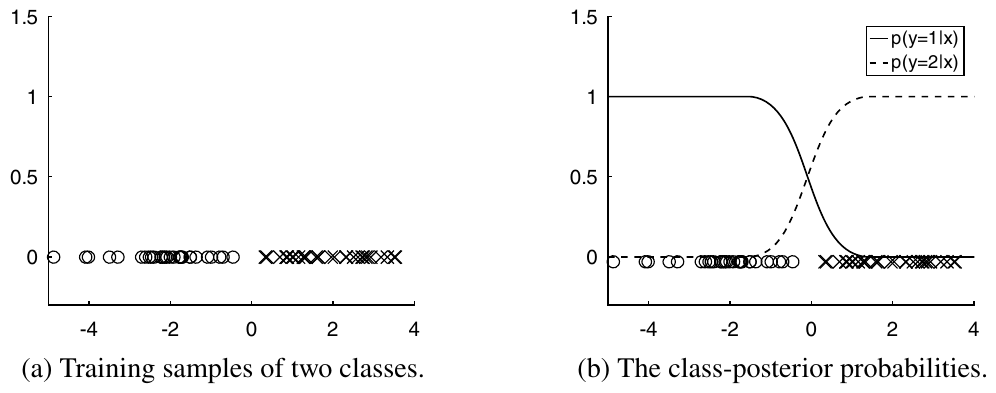
\includegraphics[width=.92\linewidth]{figures/classification-result.png}
\caption{{最小二乘概率分类的结果. (a) 两类训练样本. (b) 类别后验概率.}}\label{fig:classification-result}\end{figure}
% block: classification-result-discussion page:75 type:ordinary-paragraph
{Fig.\ \ref{fig:classification-result}a 显示前述两类样本的分布, Fig.\ \ref{fig:classification-result}b 为对应结果. 由 Fig.\ \ref{fig:classification-result}b 可见, 点 $x=0$ 属于类别 1 ($y=1$) 的概率约为 50\%, 即 $p(y=1|x=0)\approx0.5$.}
